\documentclass[a4paper,11pt]{article}
\usepackage[margin=2cm]{geometry}

\usepackage[titletoc,toc,title,page]{appendix}
\usepackage[nodayofweek]{datetime}
\usepackage{cite}
\usepackage{graphicx}
\longdate

\usepackage{minted}
\usepackage{titlesec}
\usepackage{hyperref}
\usepackage{fancyhdr}
\pagestyle{fancyplain}
\fancyhf{}
\lhead{\fancyplain{}{M.Sc.\ Group Project Report}}
\rhead{\fancyplain{}{\today}}
\cfoot{\fancyplain{}{\thepage}}


\title{Implementation of attentional bistability of the dragonfly visual neurons in an intelligent biomimetic agent\\\Large{--- Final Report ---}}
\author{Juan Carlos Farah, Panagiotis Almpouras, Ioannis Kasidakis, Erik Grabljevec, Christos Kaplanis\\
       \{jcf214, pa512, ik311, eg1114, ck2714\}@doc.ic.ac.uk\\ \\
       \small{Supervisors: Professor Murray Shanahan, Zafeirios Fountas, Pedro Mediano}\\
       \small{Course: CO530/533, Imperial College London}
}

\begin{document}
\maketitle
\section{Elementary Small Target Motion Detector}
\subsection{Methodology}

In our initial specification, one of our tasks was to connect the retina of our dragonfly to the CSTMD neurons. Having researched how this occurs in real dragonflies, we discovered that we would have to include a layer of neurons that preprocesses the input from the retina before passing it on to the CSTMDs, named elementary small target motion detectors (ESTMD) (WIEDERMAN 2008). While one of the purposes of the CSTMD seems to be to give the ability to select one target among many in the visual field (WIEDERMAN 2013), the function of the ESTMDs seems to be that of identifying small moving targets, even against a cluttered, moving background (WIEDERMAN 2008).

Our research revealed that the ESTMDs actually consist of several layers of neurons required to perform their function, namely photoreceptors, large monopolar cells (LMCs) and rectifying transient cells (RTCs) (WIED 2008). It was immediately obvious to us that implementing all these stages in a multi-compartmental model (the method used for the CSTMD) would be extremely complicated and computationally expensive. Our initial thought was to attempt to use simplified point neuron models (such as Integrate-and-fire) to achieve the ESTMD function, but with a little more research we discovered that it would be possible to do it in a simpler and more computationally efficient way using a series of spatial and temporal transforms on the retina input (WIEDERMAN 2009, HALUPKA 2013). The overview of the model we implemented is summarised in Figure 1 and the details of the transforms were taken from (HALUPKA 2013). 
One significant challenge was understanding the transforms and implementing them in Python. Understanding the transforms required some background reading on z-transforms, which are the discrete equivalent of Laplace transforms, which are necessary as our system works in discrete time steps. 
\begin{figure}
\centering
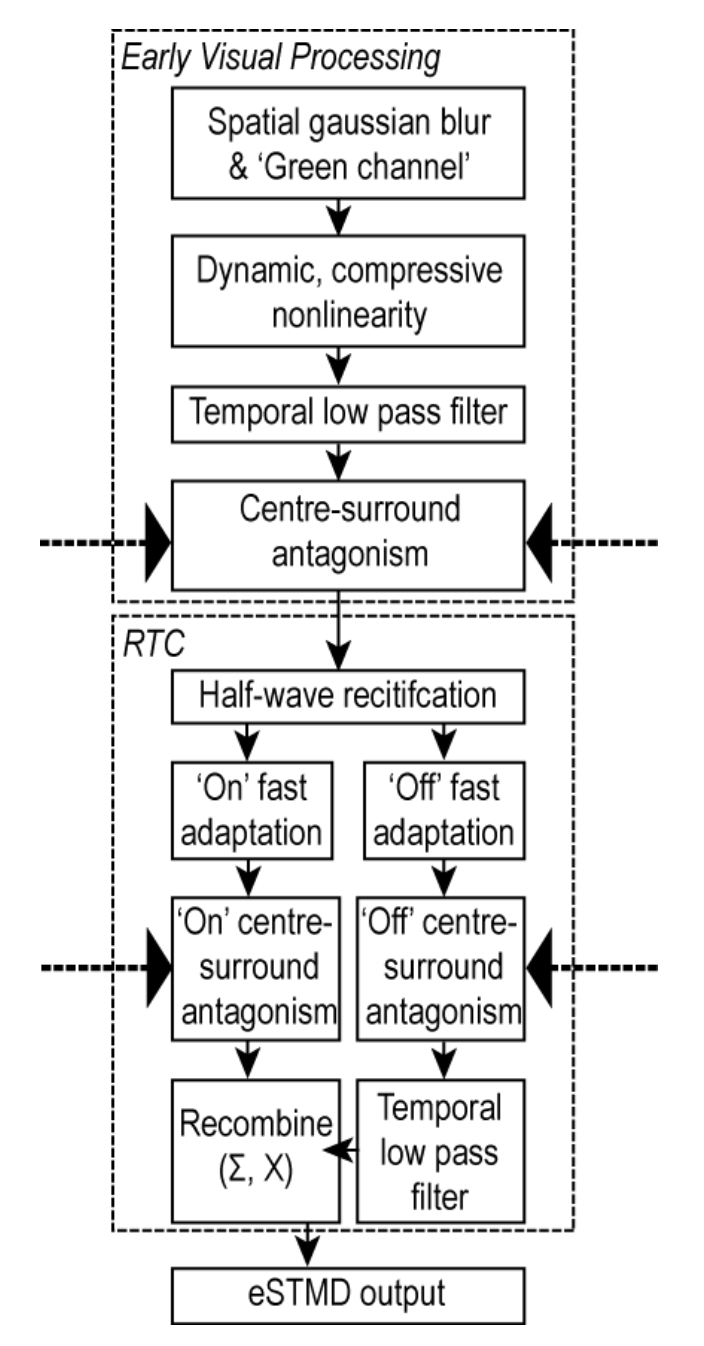
\includegraphics[scale = 0.5]{wiederman09}
\caption{CITE WIEDERMAN 2009}
\end{figure}



\end{document}
